\subsection{k-means}
\begin{figure}
    \begin{minipage}{0.5\textwidth}
        \centering
        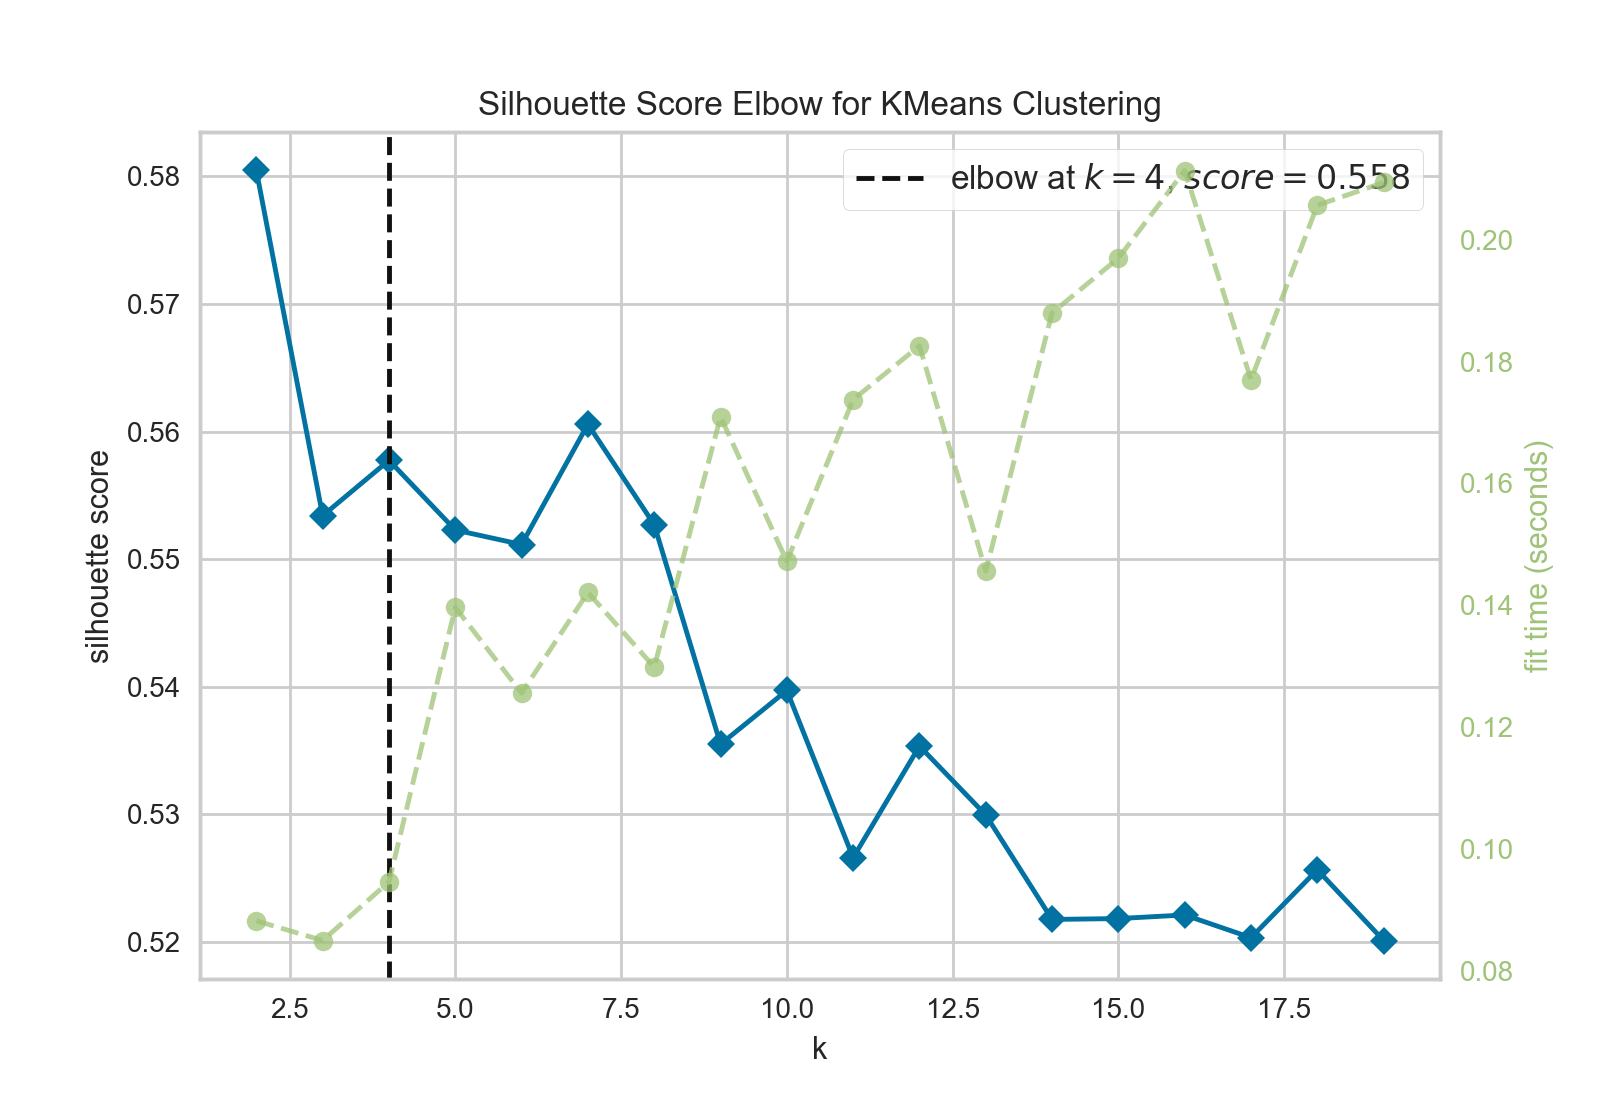
\includegraphics[width=.9\linewidth]{elbowds1.png}
        \caption{Timing curve vs silhouette coeff. dataset 1}\label{Fig:K-means vs silhouette coeff. dataset 1}
    \end{minipage}\hfill
    \begin{minipage}{0.5\textwidth}
        \centering
        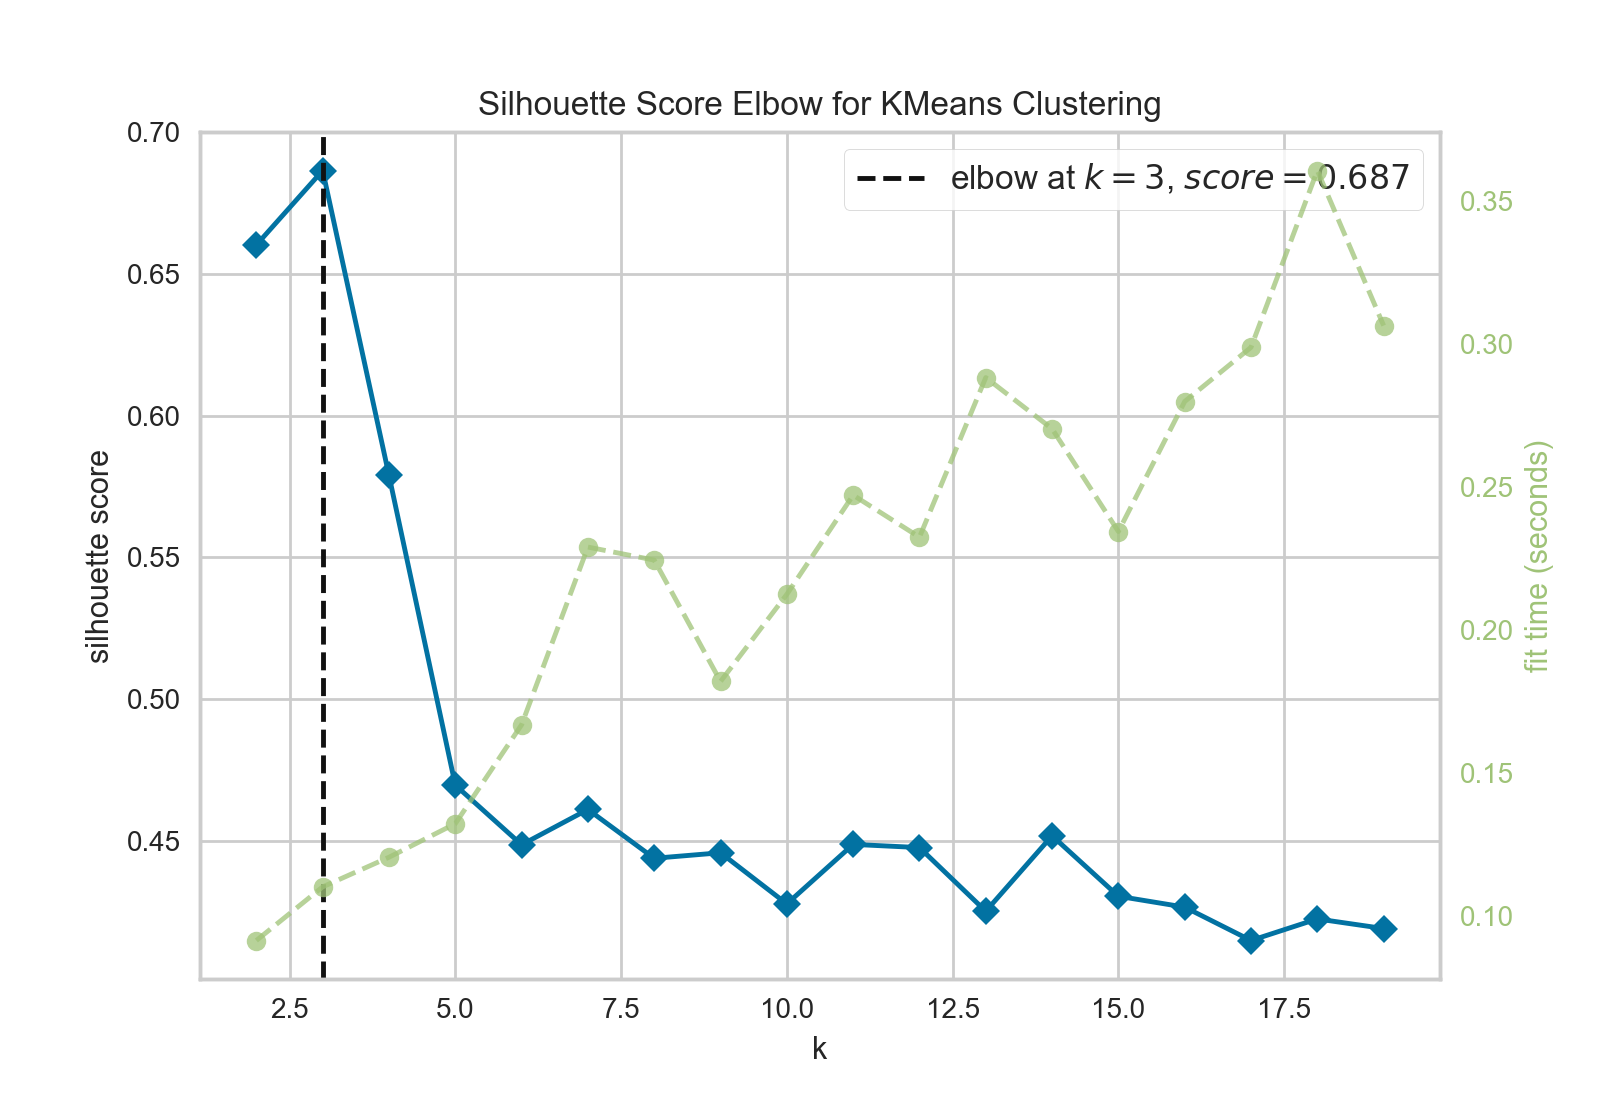
\includegraphics[width=.9\linewidth]{elbowds2.png}
        \caption{Timing curve vs silhouette coeff. dataset 2}\label{Fig:K-means vs silhouette coeff. dataset 2}
    \end{minipage}
\end{figure}
The two clustering techniques I explored for these datasets are K-Means clustering and Gaussian Mixture Models (Expectation Maximization)
In order to choose an appropriate $k$ to do k-means clustering, I used the elbow method\cite{developers_2020}.
Unless otherwise specified the standard distance measure I used was Euclidean distance.
Comparing all cluster cohesion metrics (mean distortion, silhouette coefficient, and Calinski-Harabasz score) here were
the elbow results:
\begin{center}
    \begin{tabular}{|c| c | c | c |}
        \hline
        & Metric                     & Cluster Count & Value \\
        \hline
        \hline
        Dataset 1 & Avg Silhouette Coefficient & 4             & 0.558 \\
        \hline
        Dataset 2 & Avg Silhouette Coefficient & 3             & 0.687 \\
        \hline
    \end{tabular}
\end{center}
Looking at figure~\ref{Fig:K-means vs silhouette coeff. dataset 1} and figure~\ref{Fig:K-means vs silhouette coeff. dataset 2} you can
see similar numbers in terms of the best "k".
I chose silhouette coeff over the other cluster cohesion metrics because it has a bias towards preferring well separated
clusters (coeffs closer to 1), which I anticipate would improve generalization and overall accuracy during a machine
learning process where the clusters are inputs to the learner.
Dataset 2 appears to have better separation between its 3 clusters than dataset 1's 4 clusters.
Doing further silhouette analysis on DS1 reveals that the clusters when plotted on it to the surface do not appear to
have a "cluster" round shape and instead are ovular, whereas data set two had similar characteristics to data set one
except that cluster two is actually interspersed in between cluster zero and cluster one, however this was only for the
first two features and others could have had better separation/shape.
Both clustering methods On both data sets appeared to have two very strongly defined clusters, and then up to two additional weakly defined clusters.
This more or less aligns with the fact that this is a binary classification problem and that samples could be placed into one of two clusters.
The clusters were more well defined and well separated on the second dataset which also makes sense given that all supervised learning methods performed better in terms of accuracy on this dataset relative to the first.
On closer inspection, the third and fourth clusters appear to be randomly dispersed throughout the dataset to capture outliers.
These clusters likely are noise capturers.
\begin{center}
    \begin{tabular}{|c| c | c | c |}
        \hline
        & Normalized Mutual Information & Homogeneity Score & Completeness Score \\
        \hline
        \hline
        Dataset 1 & 0.001                         & 0.002             & 0.001              \\
        \hline
        Dataset 2 & 0.189                         & 0.236             & 0.158              \\
        \hline
    \end{tabular}
\end{center}
Values closer to 1 are better than 0 in the above table for each score metric.
It seems that the performance of K-means is slightly better on dataset 2 than on 1.
To improve the performance of this we would likely need to include a dimensionality reduction technique, or modify the
dataset so that clusters are more hyper-spherical and separated from each other in the feature space.

\subsection{Expectation Maximization}\label{subsec:expectation-maximization}
\begin{figure}
    \begin{minipage}{0.5\textwidth}
        \centering
        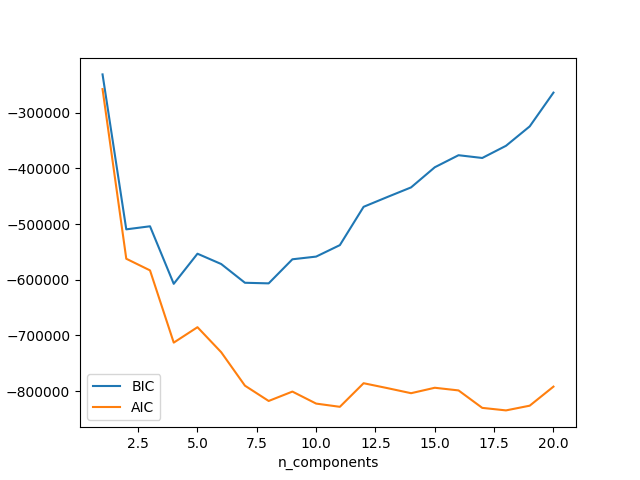
\includegraphics[width=.9\linewidth]{gmmcomponentsds1.png}
        \caption{n\_components vs AIC/BIC DS1}\label{Fig:GMM DS1}
    \end{minipage}\hfill
    \begin{minipage}{0.5\textwidth}
        \centering
        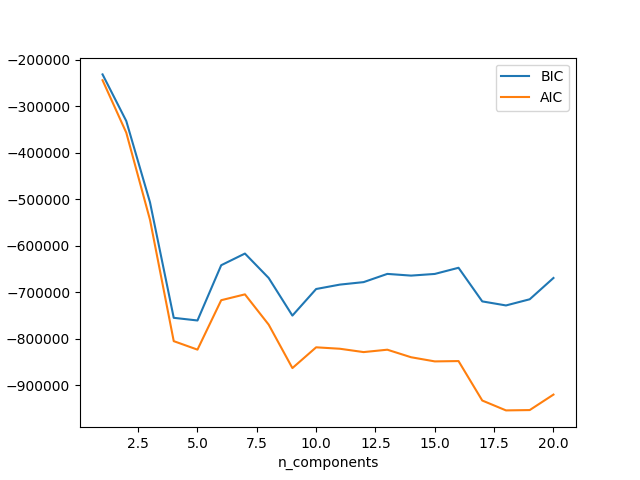
\includegraphics[width=.9\linewidth]{gmmcomponentsds2.png}
        \caption{n\_components vs AIC/BIC DS2}\label{Fig:GMM DS2}
    \end{minipage}
\end{figure}
For expectation maximization, I used the scikit-learn Gaussian mixture model function.
Based on my exploration, I do not believe that the data are distributed in a hyper-spherical format, therefore a GMM would
be able to better group samples based on its ability to accommodate non-spherical hyper-surfaces.
In order to select a best value for the number of estimators in the model, I plotted the Bayesian Information Criterion
vs the Akaike Information Criterion, where they begin to diverge is likely the best place to stop in terms of n\_estimators.
In this case looking at figures~\ref{Fig:GMM DS1} and~\ref{Fig:GMM DS2} it appears to be the same as the optimal K found
previously (4 and 3 respectively.) After finding these and running best fits and comparing results I got:
\begin{center}
    \begin{tabular}{|c| c | c | c |}
        \hline
        & Normalized Mutual Information & Homogeneity Score & Completeness Score \\
        \hline
        \hline
        Dataset 1 & 0.002                         & 0.002             & 0.002              \\
        \hline
        Dataset 2 & 0.133                         & 0.174             & 0.108              \\
        \hline
    \end{tabular}
\end{center}
These clusters more or less make sense much in the same way that K-means did.
For dataset 1, GMM outperformed in terms of mutual information, homogeneity, and completeness shared by the clustering techniques and the actual labels
whereas for dataset 2 K-means outperformed, which indicates that the data was slightly more spherical than I anticipated.
However, neither of these clustering techniques did very well since all the values were close to 0 indicating that assigment
to clusters was independent and that the clusters themselves were not very independent, nor complete.
